% FBK Science telling unofficial Bitcoin project
% 
% italian version
% 
% Bitcoin: the decentralization revolution
% 
% copyright 2014 Marco Amadori <amadori@fbk.eu>
% 
% 
% This work is released under license cc-by-sa 4.0
% 
% a copy of the license should be available within the packaging
% of this article or could be obtained from:
% http://creativecommons.org/licenses/by-sa/4.0/deed.it
% 

\documentclass[a4paper,12pt,italian]{article}


\usepackage[utf8]{inputenc}
\usepackage[T1]{fontenc}
\usepackage{textcomp}
\usepackage{lmodern}

\usepackage{gentium} % a typeface for the nations -- http://scripts.sil.org/cms/scripts/page.php?site_id=nrsi&id=Gentium

\usepackage{amsmath,amsfonts,amsthm}
\usepackage[italian]{babel}

\usepackage{hhline}
\usepackage[pdftex]{graphicx}
\usepackage{epigraph}
\usepackage{layaureo}
\usepackage{microtype}
\usepackage{fancyhdr}
\usepackage{relsize}

\usepackage[%
    colorlinks=true,%
    pdfauthor={Marco Amadori},%
    pdftitle={Bitcoin: la rivoluzione della decentralizzazione},%
    pdfdisplaydoctitle=true,%
%   hyperfootnotes=false,%
    bookmarks=true%
    ]{hyperref}

\usepackage{lettrine}
\usepackage[norule]{footmisc} % in italiano non vanno separate le note a pié di pagina
%\usepackage{creativecommons}
\usepackage{ccicons}

\usepackage{qrcode}
\usepackage[font={small,it}]{caption}
\usepackage[font=scriptsize]{subcaption}
\usepackage{wrapfig}

\setlength{\epigraphrule}{0cm}
\setcounter{DefaultLines}{3}
\renewcommand{\LettrineFontHook}{\color[gray]{0.5}}

\pagestyle{fancy}
\rfoot{\ccbysa}
\lhead{\scshape Bitcoin: la rivoluzione della decentralizzazione}

\makeatletter
\renewcommand\maketitle{
\newpage\thispagestyle{empty}
    \begin{center}
        {\huge\@title\par}
        \bigskip
        {\ttfamily \today{}\par}
    \end{center}
}
\makeatother

\newcommand{\qrfig}[1]{%
 \centering%
 \subcaptionbox{\url{#1}\bigskip}[.3\linewidth]{%
 \qrcode[height=2.6cm]{#1}}%
}

\newcommand{\longurl}[1]{%
\href{#1}{\ttfamily \smaller #1}%
}%

%\DeclareCaptionSubType[arabic]{figure}
\captionsetup[figure]{labelformat=empty}
\captionsetup[subfigure]{labelformat=empty}


\title{\textbf{Bitcoin: la rivoluzione della decentralizzazione} \\ 
  \bigskip
  \begin{Large}Come la moneta digitale volontaria 
  porterà un’ondata di innovazione dirompente
  \end{Large}
}


\date{\vspace{-5ex}}
\author{\vspace{-5ex}}
\author{\begin{small}Marco Amadori \href{mailto:amadori.fbk.eu}{<amadori@fbk.eu>} \\ 
Tecnologo e Ricercatore presso FBK
\end{small}}



\begin{document}
\maketitle

\epigraph{\textit{Da qui al 2005, diverrà chiaro che l’impatto di Internet sull’economia
non sarà stato più grande di quello del fax.}\footnotemark}{\bigskip
1998 --- Paul R. Krugman \\ 
Premio Nobel per l’economia 2008}

\footnotetext{\href{http://www.businessinsider.com/paul-krugman-responds-to-internet-quote-2013-12}
{\url{http://web.archive.org/web/19980610100009/www.redherring.com/mag/issue55/economics.html}}}

\section*{La rivoluzione dal basso}

\lettrine{È}{ possibile che dalle idee di un perfetto sconosciuto} parta un fenomeno
nuovo che in pochi anni vada a perturbare le agende di Governi e
Istituzioni Finanziarie a livello globale?

\bigskip

Sì, se lo sconosciuto è \emph{Satoshi Nakamoto} e il fenomeno si chiama
\emph{Bitcoin}.

\bigskip

Il termine “rivoluzione” è spesso usato in contesti inappropriati, per
il marketing \emph{un prodotto è rivoluzionario}, per un partito politico una
proposta di legge è rivoluzionaria, per i tecno-entusiasti \emph{un
telefonino può essere rivoluzionario}. Ma se togliamo il termine da
questi contesti dove può suonare esagerato quando non ridicolo,
immagineremo probabilmente sommosse popolari, sangue e violenza. Per il
\emph{Wikizionario} (anni fa avremmo citato il \emph{Devoto-Oli}) la “rivoluzione” è
un “improvviso \emph{cambiamento di idee}, condizioni sociali, economiche,
culturali, politiche in forte contrapposizione a quelle
precedenti”\footnote{Enfasi dell'autore: \url{http://it.wiktionary.org/wiki/rivoluzione}}.

\bigskip

L’energia elettrica è stata rivoluzionaria, il motore a scoppio lo è
stato, il computer sicuramente. Ma questi furono cambiamenti accettati
come \emph{rivoluzionari solo dai posteri}; quando l’innovazione arrivò nel
sistema per la prima volta l’atteggiamento fu molto diverso. Per fare
un esempio: i primi proprietari di auto in Inghilterra dovevano per
legge avere a bordo un pilota, un ingegnere e una persona con una
bandierina con il compito di precedere il mezzo di trasporto e fare largo tra
carri e pedoni. \emph{I primi automobilisti erano} dunque visti come degli
eccentrici, \emph{dei pazzi che rischiavano la vita} con macchinari puzzolenti
che procedevano a passo d’uomo e che non avevavo proprie strade dove
essere usati.

\begin{wrapfigure}{R}{.6\linewidth}
\centering
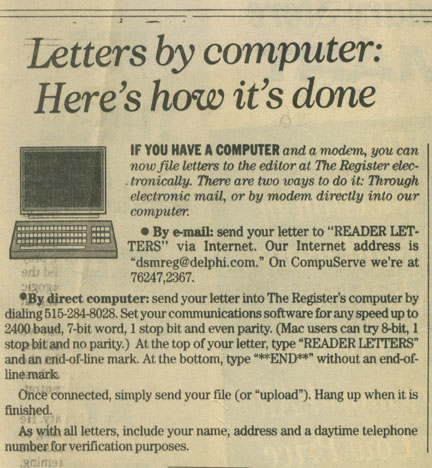
\includegraphics[width=.9\linewidth]{figures/pc_news.jpg}
\caption{Interfacce amichevoli -- User friendlyness.}
\vspace{-10pt}
\end{wrapfigure}

Per citare tempi più recenti, quanto poteva sembrare
 \emph{assurda l’idea stessa dell’email} ad un comune cittadino italiano nei
primi anni ‘90? Serviva un computer da circa 2 milioni di lire, un
modem quasi altrettanto costoso ed una connessione ad Internet, magari
presso un provider che avrebbe richiesto una carissima telefonata
interurbana per connettersi; peggio ancora, anche il nostro
destinatario avrebbe dovuto avere una configurazione compatibile con la nostra.
\bigskip

La rivoluzione, mentre accade, non è quasi mai vissuta dai contemporanei per
quello che è, c’è sempre una forza, di abitudine, di stasi, di mancanza
di fantasia, che si oppone al cambiamento.
\bigskip



Siamo ora in una fase di questo tipo, dove è da poco arrivato uno strumento di 
\emph{innovazione dirompente} che fa leva su una \emph{tecnologia rivoluzionaria}:
il \emph{Bitcoin}\footnote{\url{https://bitcoin.org/it/}}; ma andiamo con ordine.


\section*{La nascita del Bitcoin}



\lettrine{I}{l 31 Ottobre del 2008} veniva
postato\footnote{\url{http://www.metzdowd.com/pipermail/cryptography/2008-October/014810.html}} 
su una mailing list di crittografia un pdf che sta cambiando permanentemente
 il paradigma monetario e finanziario nel quale siamo immersi fin
dai tempi antichi. Cioè che la moneta dev’essere di proprietà di un
Autorità Superiore, sia essa lo Stato, il Sovrano o una Banca Centrale.
Il pdf si intitolava “\emph{Bitcoin: A Peer-to-Peer Electronic Cash
System}”\footnote{Originale: \url{https://bitcoin.org/bitcoin.pdf}, e traduzione
in italiano: \url{https://docs.google.com/file/d/0B1UsG65HCLkuMjA3Mzk2ZTUtYjQ4Ni00MjEyLTgzN2ItMjI3ODU0M2Y4MGUx/edit}
} e definiva il funzionamento di una moneta digitale, decentralizzata, non controllata
da un ente ed emessa in base ad un algoritmo.

\smallskip

L’accettazione tra i crittografi che seguivano la mailing list non fu
unanime, anzi, l’incredulità era forse il sentimento più diffuso. Del
resto non possiamo biasimarli, anch’io la prima volta che lessi di
Bitcoin pensai solamente che fosse un’idea curiosa, divertente, \emph{un
giochino intellettuale per nerd} e poco altro. Il problema
d’accettazione del Bitcoin deriva dal fatto che non solo veniva
introdotto un concetto al quale non siamo abituati, cioè una l’idea di
\emph{una moneta} non a corso legale ma \emph{ad uso volontario}, ma anche dalla
ragione che per farlo, Satoshi aveva creato un sistema informatico che
non aveva precedenti: la tecnologia del \emph{registro delle transazioni
distribuito} permetteva funzionalità mai state prima disponibili in
informatica e la moneta digitale era solo una prima applicazione di
tale tecnologia.


\bigskip

Monete digitali erano esistite anche prima, c’era stato
l’\emph{e-gold}\footnote{\url{http://en.wikipedia.org/wiki/E-gold}}, i
\emph{beenz}\footnote{\url{http://en.wikipedia.org/wiki/Beenz.com}}, i \emph{liberty
dollars}\footnote{\url{http://en.wikipedia.org/wiki/Liberty\_Dollar}},
tutti progetti centralizzati che erano in diversi modi naufragati o
fatti naufragare, perché \emph{avevano un unico punto di vulnerabilità}
(\emph{single point of failure}) ed erano facilmente attaccabili o delicati.
Satoshi probabilmente pensò alla differenza tra Napster\footnote{\url{http://it.wikipedia.org/wiki/Napster}},
altra tecnologia dirompente, e Bittorrent\footnote{\url{http://it.wikipedia.org/wiki/BitTorrent}};
il primo, centralizzato era stato
chiuso da una banale operazione dell’FBI, mentre Bittorrent,
decentralizzato, si era già dimostrato non solo inarrestabile, ma anche
\emph{antifragile}. Il termine \emph{antifragile}, significa che più una cosa viene
attaccata e più diventa resistente; è una proprietà che il bitcoin ha \textit{di progetto}.\footnote{
\url{http://bitcoin.stackexchange.com/questions/11867/is-bitcoin-antifragile}}

Tenendo chiari gli \emph{svantaggi di corruttibilità} e \emph{fallibilità}, la \emph{centralizzazione} 
ha anche alcuni vantaggi rispetto alla \emph{decentralizzazione}. La decentralizzazione è spesso più
complessa e meno efficiente: una monarchia assoluta è tecnicamente un sistema
più semplice di una democrazia. 

\smallskip


Nel caso di una moneta digitale, una \emph{terza parte autorevole} permette di evitare la spesa multipla
di uno specifico oggetto digitale (es. un ammontare di bitcoin) tenendo un solo registro, un solo \emph{libro mastro delle transazioni}, su 
un sistema informatico centrale, a costi minori di un sistema decentrato. Ma la complessità del sistema fiduciario necessario per 
regolare l'accesso a questa unica risorsa di controllo, può essere molto costosa da manutenere ed eclissare anche i pochi vantaggi di efficienza potenziale.

\smallskip
Essendo nel
mondo digitale, poco costoso effettuare \emph{copie perfette}, \emph{come si
può evitare di copiare} perfettamente \emph{del denaro digitale} senza fare uso di un'autorità centrale
che permetta di evitare una spesa multipla (\emph{double spend} problem)?


\smallskip

Satoshi si appropriò di strumenti informatici preesistenti e li assemblò
in maniera innovativa: usò la \emph{crittografia}\footnote{\textsc{ecdsa}, firma
crittografica a curva ellittica di tipo secp256k1, 
\longurl{http://en.wikipedia.org/wiki/Elliptic\_Curve\_Digital\_Signature\_Algorithm
}.} per firmare digitalmente le transazioni, da
Bittorrent prese
l’idea e la tecnologia per ottenere \emph{il libro mastro distribuito} come se
fosse un file di un film in condivisione e infine, da un progetto
pensato per ridurre lo spam nelle email\footnote{\emph{Hashcash},
\url{http://en.wikipedia.org/wiki/Hashcash}}, prese l’idea di associare una
quantità di lavoro crittografico\footnote{\emph{Proof of Work}, il lavoro
crittografico è una ripetizione di una funzione hash (double sha256)
dello stato delle transazioni degli ultimi 10 minuti. Vedi
\url{http://it.wikipedia.org/wiki/Proof-of-work}. Questo meccanismo è usato in un nuovo 
tipo di \emph{firma crittografica}, la ``\textsc{dmms}'', \emph{Dynamic-Membership Multiparty Signature}, per la
prima volta delineata nell'articolo sulla tecnologia delle \emph{sidechains}: \url{http://www.blockstream.com/sidechains.pdf}}, cioè energia
elettrica trasformata in calcoli, e di \emph{usare questo lavoro come se
fosse un voto} in una democrazia (da una testa uguale un voto ad \emph{un calcolatore
uguale un voto}) per \emph{stabilire il consenso in una rete di computer}.\footnote{Per
spiegazioni più dettagliate su questo funzionamento, l’articolo
originale di Satoshi risulta una fonte chiara e sufficientemente
accessibile.}
Per l'uso massiccio di strumenti crittografici le valute come il Bitcoin vengono ora generalmente chiamate
\emph{crittovalute} (\emph{crypto-currencies}) o anche \emph{monete matematiche}.


\section*{La crescita esponenziale}


\lettrine[lines=2]{D}{ifficile riuscire ad immaginare} il futuro in prospettiva, molto più
facile è fare una retrospettiva. Che cosa è successo in questo ultimo
anno al progetto Bitcoin?

In questa tabella 
si vedono alcuni parametri relativi all'ultimo anno (2013); i negozi online e fisici
che accettano Bitcoin sono esplosi, i \emph{bancomat bitcoin} (\textsc{btm}, 6 in
Italia, con altri in arrivo) erano un fenomeno sconosciuto, l’\emph{Hash Rate}
globale, che è una misura della sicurezza della rete, è aumentato di
216 volte. La crescita dei progetti \emph{Github}\footnote{\url{https://github.com/}}
significa che gli sviluppatori software stanno lavorando sempre più per
produrre strati tecnologici, servizi e nuovi modi di usare la
tecnologia Bitcoin per usi impensabili (qualcuno lo citerò più
avanti).

\begin{figure}
\centering
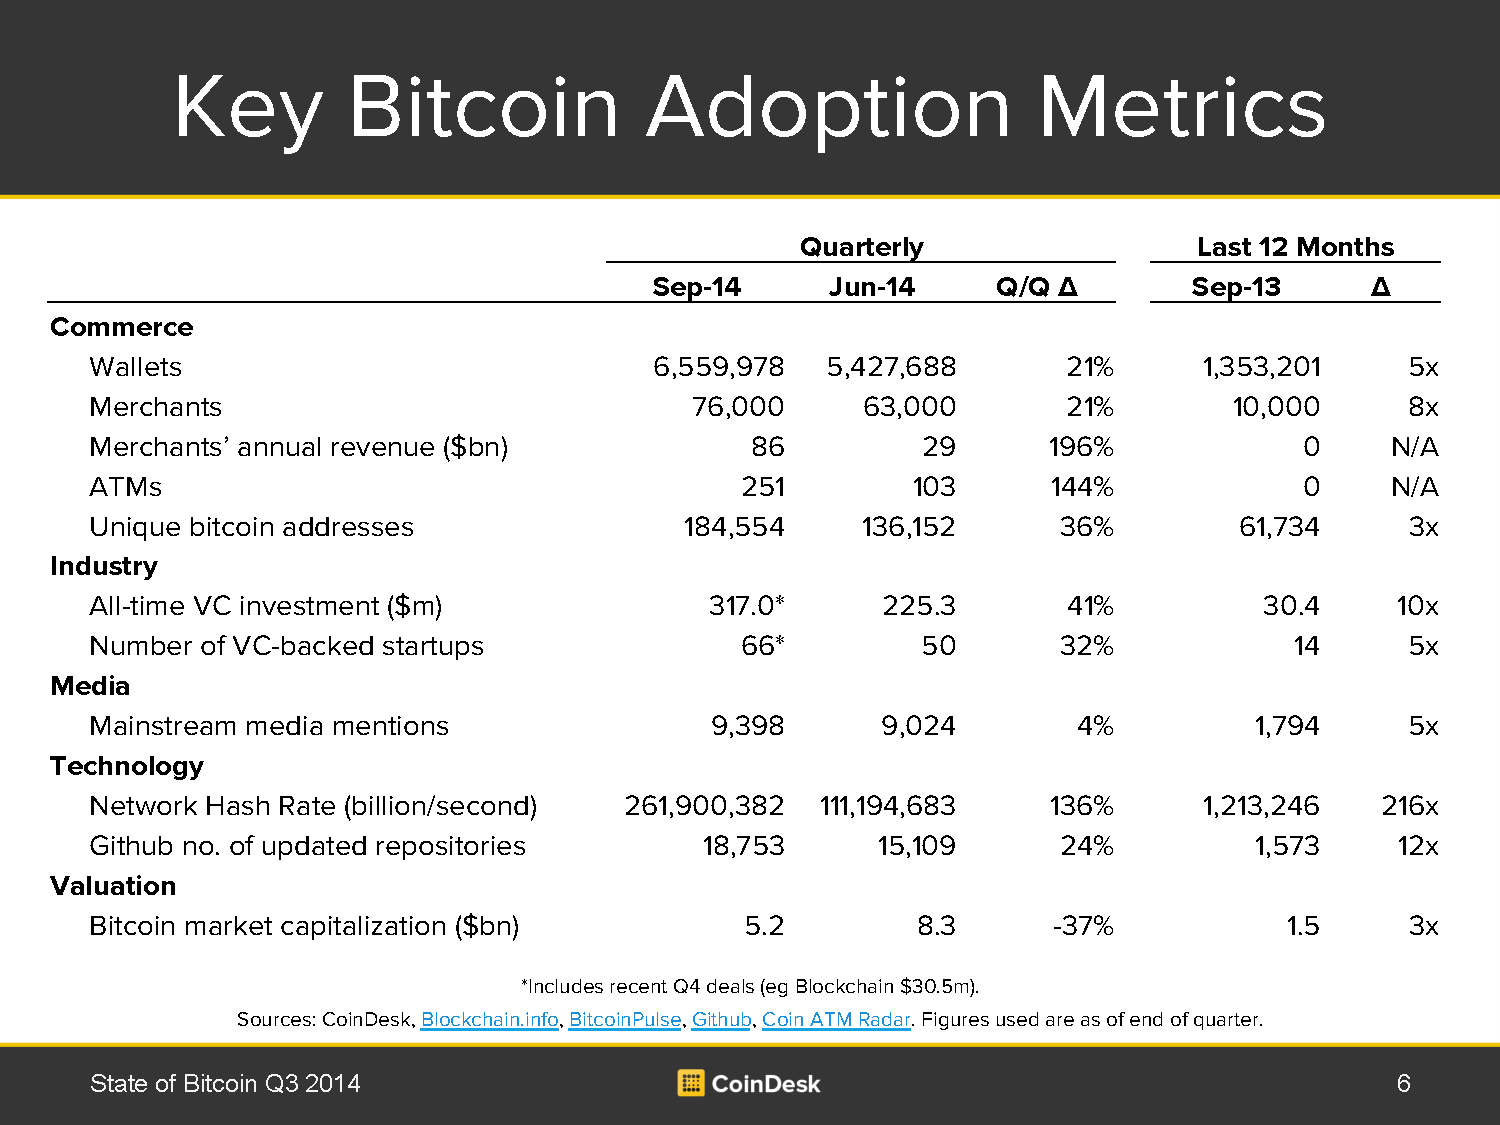
\includegraphics[width=.8\linewidth]{figures/metrics.pdf}
\caption{Report trimestrale Q3 2014 -- redatto da \url{http://www.coindesk.com}}
\end{figure}



\subsection*{Quanto costa un bitcoin}


Il bitcoin è un bene \emph{scarso}, ce ne sono in circolazione 13 milioni circa
e al massimo nel 2140 ce ne saranno \emph{21 milioni, non uno di più}. Un
bitcoin, ad oggi sul finire del 2014, è scambiato per circa 300 €, ma se ne possono
possedere anche delle frazioni, essendo divisibile in 100 000 000 
unità (chiamate come il creatore, “satoshi”)\footnote{Ultimamente
la community di bitcoiners sta spingendo per utilizzare un
sottomultiplo del bitcoin, cioè il “bit” che equivale a un milionesimo
di bitcoin, o in altri termini 100 \emph{satoshi}, in modo da avere solo 2
decimali invece di 8, come capita per le monete tradizionali a corso
forzoso alle quali siamo abituati; l’idea del cambiare il riferimento
di base nasce dalla constatazione che dovremmo trovare più facile a
pagare un caffé 3000 bits piuttosto che 0.003 bitcoin. 
}.

\smallskip

Il prezzo del bitcoin \emph{è dato unicamente dal Mercato}, seguendo le leggi della domanda e
dell'offerta. Esistono diversi cambiavalute, che siano essi attrezzature simil-bancomat,
persone fisiche o servizi online (\emph{exchange}), che permettono di \emph{vendere e comprare bitcoin per} valuta a
corso forzoso come \emph{euro o dollari} (chiamate tecnicamente \emph{fiat currencies}).
In questa fase iniziale lo scambio del bitcoin per \emph{valuta fiat} comporta
che il prezzo sia molto \emph{volatile}\footnote{
La \emph{volatilità} è la proprietà di un bene di essere soggetto a variazioni
percentualmente significanti del prezzo nell'arco del tempo; il bitcoin può ancora 
esprimere variazioni dell'ordine del 10\% nell'arco di una giornata.},
ma è una peculiarità che è destinata
naturalmente a diminuire mentre l’adozione continua. Pensate che il
primo scambio, ormai famoso, tra un bene e bitcoin è avvenuto nel 2010, dove una
persona scambiò 10 000 bitcoin per due pizze\footnote{\url{https://bitcointalk.org/index.php?topic=137.0}}
a domicilio, fissando
impropriamente una quotazione del bitcoin a circa 0.002 € (supponendo
20 € per due pizze); quella stessa quantità ora vale circa 3 milioni di
euro.\footnote{\url{https://duckduckgo.com/?q=10000+bitcoin+euro}}

\begin{figure}
\centering
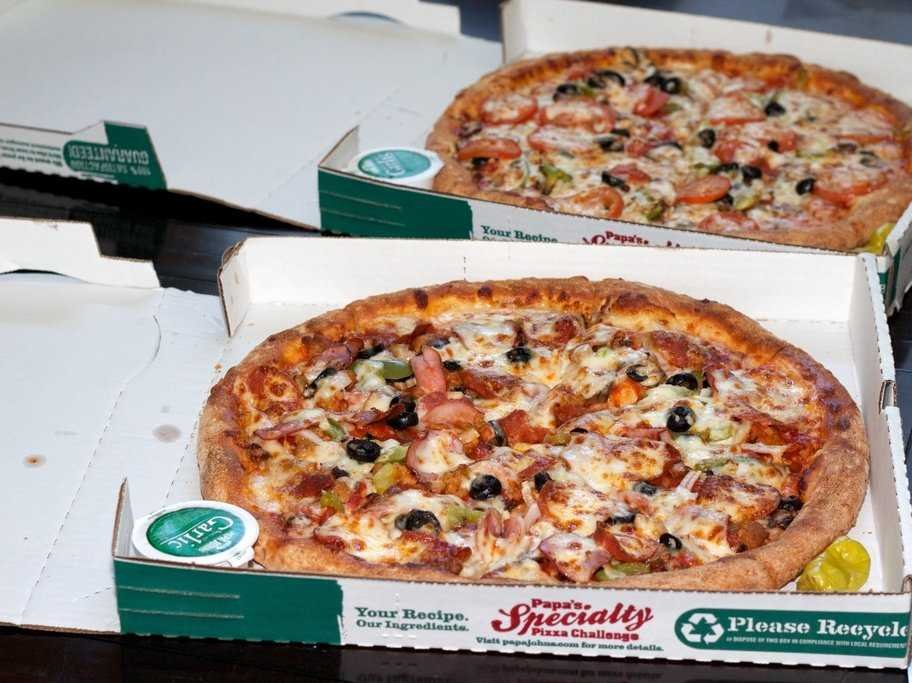
\includegraphics[width=.8\linewidth]{figures/laszlo_pizzas.jpg}
\caption{10 000 bitcoin, le pizze più costose della storia.}
\end{figure}


Com’è potuto crescere il prezzo di più del 100 000\% in qualche
anno?

\bigskip


Il perché questo avvenga è semplice, perché \emph{il bitcoin è utile, ma
scarso}.
\bigskip


\emph{Non se ne possono stampare di più}, la loro \emph{creazione} dipende solo
dall’algoritmo e viene generata in maniera \emph{predicibile} e \emph{distribuita} da
chi partecipa con risorse di calcolo alla sicurezza della rete (chi fa
questo usa computer specializzati che vengono chiamati “miner”\footnote{Nel 2012 si poteva fare \emph{mining}
anche con un PC tradizionale, ma il fenomeno è stato così profittevole da far sì che venisse
sviluppata una tecnologia specifica per il \emph{mining}. Ora per \emph{minare} servono delle attrezzature 
ottimizzate basate non su processori generici da PC e nemmeno GPU delle schede video, ma su degli \textsc{asic} -- Application
Specific Integrated Circuit -- dei processori che eseguono solo la funzione necessaria al \emph{mining} di bitcoin.
}). Va da
sé che più si diffonde il fenomeno (sia tra gli utenti, che come
tecnologia) e più ne aumenta il prezzo, perché, a fronte di
un’emissione in costante declino, una domanda statica o in crescita
porta ad un aumento del prezzo di ciascun bitcoin. Ma gli aspetti
speculativi sono marginali rispetto all’utilità sia del Bitcoin come
valuta che della tecnologia sottostante.

\begin{figure}
\centering
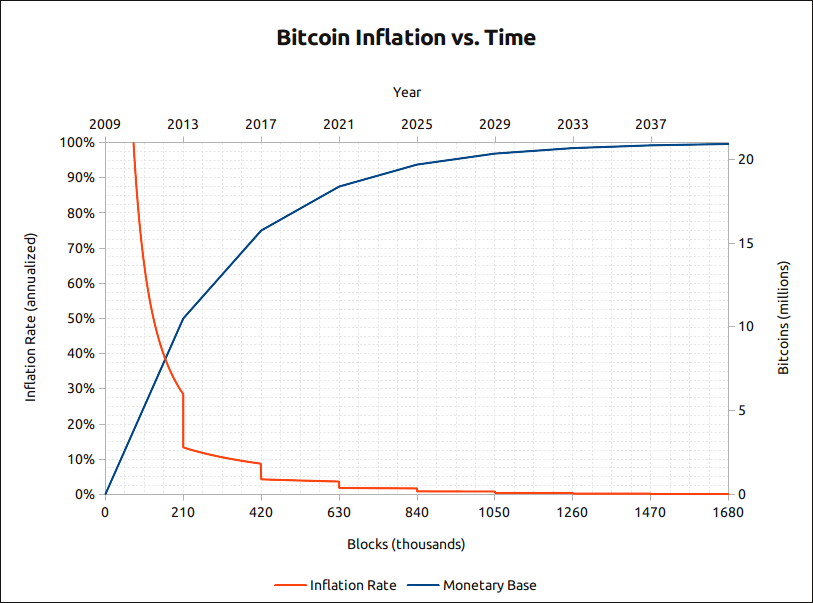
\includegraphics[width=\linewidth]{figures/inflation.png}
\caption{Creazione di nuova moneta nel tempo, chiamata \emph{inflazione} monetaria (non dei prezzi al consumo).}
\end{figure}


\section*{Il Bitcoin come valuta}


\lettrine{P}{er capire che cosa è} il Bitcoin come strumento per trasmettere valore,
senza addentrarci in tecnicismi complicati (chi di voi mentre legge
queste righe sa esattamente come funziona il protocollo \textsc{tcp/ip} o il
linguaggio di markup \textsc{html} che rende il web possibile?) usiamo una
metafora presa in prestito proprio da Satoshi:

\begin{quotation}
\noindent
\emph{Immaginate un metallo simile all’oro} quanto a scarsità di presenza
sulla superficie terrestre\footnote{170 000 tonnellate estratte sin dagli
albori dell’umanità.} e quanto a difficoltà di estrazione. Immaginatelo
però di un colore grigiastro per nulla attraente, né duttile né
malleabile, privo di funzioni ornamentali o costruttive, che non sia né un buon
conduttore elettrico, ma nemmeno un buon isolante, brutto a
vedersi al posto di un dente (va be' che già
l'oro\ldots NDA), insomma, \emph{del tutto inutile}.

\smallskip

\noindent
Però con una magica proprietà, cioè che \emph{può essere trasmesso 
attraverso un canale di comunicazione}.\footnote{Libera traduzione da:
\url{https://bitcointalk.org/index.php?topic=583.msg11405\#msg11405}}
\end{quotation} 


\bigskip

Capirete che un metallo del genere potrebbe avere un ruolo notevole per
la trasmissione a distanza di potere d’acquisto.

\subsection*{Del resto che cos’è una moneta?}

\lettrine{S}{econdo la definizione di Aristotele}, la moneta doveva essere un
bene \emph{non deperibile}, \emph{scarso} (cioè disponibile in \emph{quantità limitata}),
facilmente \emph{divisibile} e con \emph{valore intrinseco}.
Secondo definizioni moderne è moneta ciò che può essere usato come
mezzo di \emph{trasmissione del valore}, come \emph{unità di conto} e come \emph{riserva di
valore}. 

\smallskip

Secondo entrambe queste definizioni il nostro euro non è
proprio una moneta esemplare, perché riguardo la prima definizione
manca di \emph{valore intrinseco o valore d’uso}, cioè non ha altra utilità se non quella di
scambio, mentre rispetto alla seconda definizione come riserva di
potere d’acquisto, sul lungo periodo non si comporta molto bene, basti
pensare a quanto si poteva acquistare 30 anni fa con 100 000 lire e
paragonarle al potere d’acquisto degli attuali 50 €. La mancanza di
valore d’uso della moneta \emph{fiat} non è un problema fondamentale, visto
che in realtà il valore d’uso non serve a molto se non come avvio del
fenomeno, pensiamo per esempio all’oro o alle conchiglie, monete del
passato, che avevano anche usi ornamentali che ne stimolavano la
domanda iniziale.


\bigskip

Il bitcoin è una \emph{moneta volontaria}. Chiunque può scambiarla e accettarla
senza chiedere il permesso o a nessuno (\emph{permissionless}). Le transazioni sono \emph{permanenti},
\emph{irreversibili} e con tariffe bassissime o nulle, in generale si parla di
0.3 centesimi di euro a transazione (che sia essa di un euro o di un
milione di euro).

\smallskip
Per poter accettare bitcoin è sufficiente crearsi un indirizzo bitcoin
all'interno di una delle tante applicazioni software
gratuite disponibili online\footnote{
Un esempio di \emph{wallet} online sicuro e versatile è \url{https://greenaddress.it/it/}},
chiamate \emph{wallet} o \emph{portafogli}\footnote{Sarebbe più corretto chiamarle \emph{portachiavi},
visto che memorizzano e gestiscono delle \emph{chiavi private}, ma gli ingegneri non sono sempre a loro agio con le metafore.}; detto
indirizzo, un numero di 256 cifre binarie quasi sempre rappresentato da
una strana sequenza di numeri o lettere (es.
\texttt{\begin{scriptsize}1FBKmAA3gFzuT28MpA4EfuqQ5kJEFS9owS\end{scriptsize}}) svolge la funzione del tradizionale
conto corrente bancario, senza tuttavia che siate costretti ad aprire
uno presso alcuna banca. Con Bitcoin infatti si può diventare banche di
noi stessi.


\bigskip

Il Bitcoin (con la “B” maiuscola) indica invece il protocollo, il codice
Open Source che permette di implementarlo e la rete peer-to-peer dove
vengono trasmesse le transazioni.

\bigskip

Bitcoin è questione di libertà. Le transazioni possono essere \emph{anonime} a
piacere \emph{o trasparenti a piacere}, dato che il libro mastro delle
transazioni, chiamato \emph{Blockchain}, è pubblico e chiunque può vedere
tutte le transazioni avvenute dal primo blocco iniziale, il \emph{Genesis
Block}\footnote{
\longurl{https://blockchain.info/it/tx/4a5e1e4baab89f3a32518a88c31bc87f618f76673e2cc77ab2127b7afdeda33b}}, ad oggi.
\emph{Le transazioni avvengono tra pseudonimi}, cioè gli
indirizzi bitcoin, da quello del mittente a quello del destinatario; se
però ad esempio rendessi pubblico sul mio blog personale il mio
indirizzo bitcoin, permettendo di associarlo alla mia persona, ecco che
dall’anonimato scaturirebbe una funzionalità inaspettata e dirompente:
\emph{la trasparenza}.

\begin{figure}
\centering
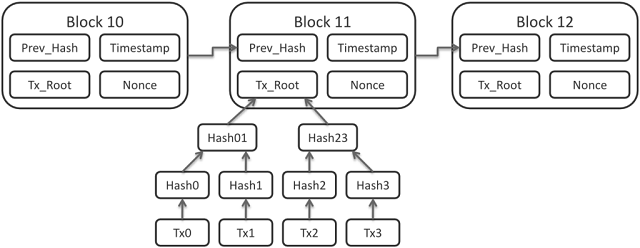
\includegraphics[width=\linewidth]{figures/Bitcoin-Block-Data.png}
\caption{Un diagramma che rappresenta concettualmente la \emph{Blockchain}.}
\end{figure}

\bigskip

\section*{Il valore della trasparenza}

\lettrine{P}{ensate ad un partito politico} che pubblicasse il suo indirizzo bitcoin
per le donazioni da privati o per il ricevimento di soldi pubblici. Potrebbe
farsi vanto di avere realizzato una forma di \emph{trasparenza finanziaria
totale}. Chiunque, giornalisti e cittadini, avrebbero modo di vedere
dove fluiscono i soldi e come vengono spesi. Idem per la pubblica
amministrazione.

\smallskip

Oppure pensiamo al privato, dove un produttore di cibo biologico
mostrasse che i suoi bitcoin arrivano, veramente e ad ogni nostro
acquisto, ai fornitori di materia prima biologica \emph{certificando in
automatico la sua filiera} ad un livello oggi impensabile.


\bigskip

Parliamo di una moneta potenzialmente \emph{autotracciante}, che si
\emph{autodocumenta} in maniera pubblica. Si noti come questa funzionalità,
tra qualche tempo, potrebbe impensierire i commercialisti, il cui ruolo
ad oggi è quello di fornire dei servizi che il Bitcoin \emph{implementa
automaticamente}.


\bigskip

Ovviamente pensando ad una valuta globale, oltre alla trasparenza, la
\emph{pseudonimità} è un grande valore negli scambi \emph{tra privati}. Non possiamo
supporre che i governi o le istituzioni siano sempre benevole, ci sono
parti del mondo dove questo non è vero e la possibilità di effettuare
scambi in maniera anonima potrebbe proteggerci da aggressioni o
ritorsioni. Questo è possibile dato che \emph{l’associazione} tra indirizzo
Bitcoin ed individuo \emph{è solo volontaria}.


\bigskip

Attualmente \emph{i commercianti} che accettano bitcoin \emph{sono in forte aumento},
questo anche perché sono già mature sul mercato soluzioni che azzerano
il problema della fluttuazioni dei valori di cambio rendendolo molto
appetibile. Un negozio, con solo uno smarphone, un tablet o
semplicemente un QRcode adesivo di un indirizzo bitcoin, può accettare
questa moneta direttamente e senza rischi. Ci sono aziende, come
Bitpay\footnote{\url{https://bitpay.com/}}, che dato un prezzo in euro,
permettono ai commercianti di accettare pagamenti in bitcoin
continuando però a ricevere euro sul conto in banca, mascherando
completamente al mercante la volatilità momentanea del bitcoin e a 0\%
di tariffe, rendendo per un negoziante il Bitcoin un sistema di pagamento 
molto più vantaggioso di bancomat o carte di credito, che hanno tariffe non
trascurabili.

Limitatamente a questo ambito, i \emph{vantaggi immediati per il consumatore}, oltre alle partecipazioni ai \emph{minori costi}
dei negozianti sotto forma di promozioni, sono il \emph{non dover fornire} a terzi \emph{dati sensibili non 
necessari}, evitando di dover ``tremare'' ogni volta che si sente la notizia di dati personali o numeri di carte di credito, trafugati
da qualche sistema informatico centralizzato (ancora dei \emph{punti di vulnerabilità} dei sistemi tradizionali).


\section*{Bitcoin è globale}


\lettrine{I}{n Europa}, soprattutto nel Regno Unito, in Germania e in Olanda,
Il Bitcoin è un fenomeno generalmente più noto che in Italia, 
dove spesso purtroppo si è in ritardo sulle nuove tecnologie rispetto ai nostri cugini d'oltralpe.
Questo dicembre a Monaco, si terrà un evento per la creazione della prima banca che fornirà servizi integrati sulle
\emph{cryptovalute} come il Bitcoin\footnote{\url{https://www.cryptocurrency-bank.com/}} e la Svizzera  già da giugno ha fatto progressi per 
attirare innovazione, facendo chiarezza sulle interpretazioni tributarie, suggerendo di trattare
i bitcoin come valuta estera.\footnote{\url{http://www.coindesk.com/swiss-report-lays-foundation-bitcoin-become-legal-money/}}

Oltre allo scenario commerciale europeo, o alla febbre Bitcoin dei \emph{capitalisti di ventura} (\textsc{vc}) statunitensi che investono sulle nuove imprese Bitcoin cifre paragonabili
a quelle investite nei primi anni di Internet, ricordiamoci che il Bitcoin è un fenomeno globale, non riguarda solo l’Italia o il
benestante “occidente” ma anche il 50\% della popolazione mondiale che
non ha accesso al credito e agli strumenti bancari.

\begin{figure}
\centering
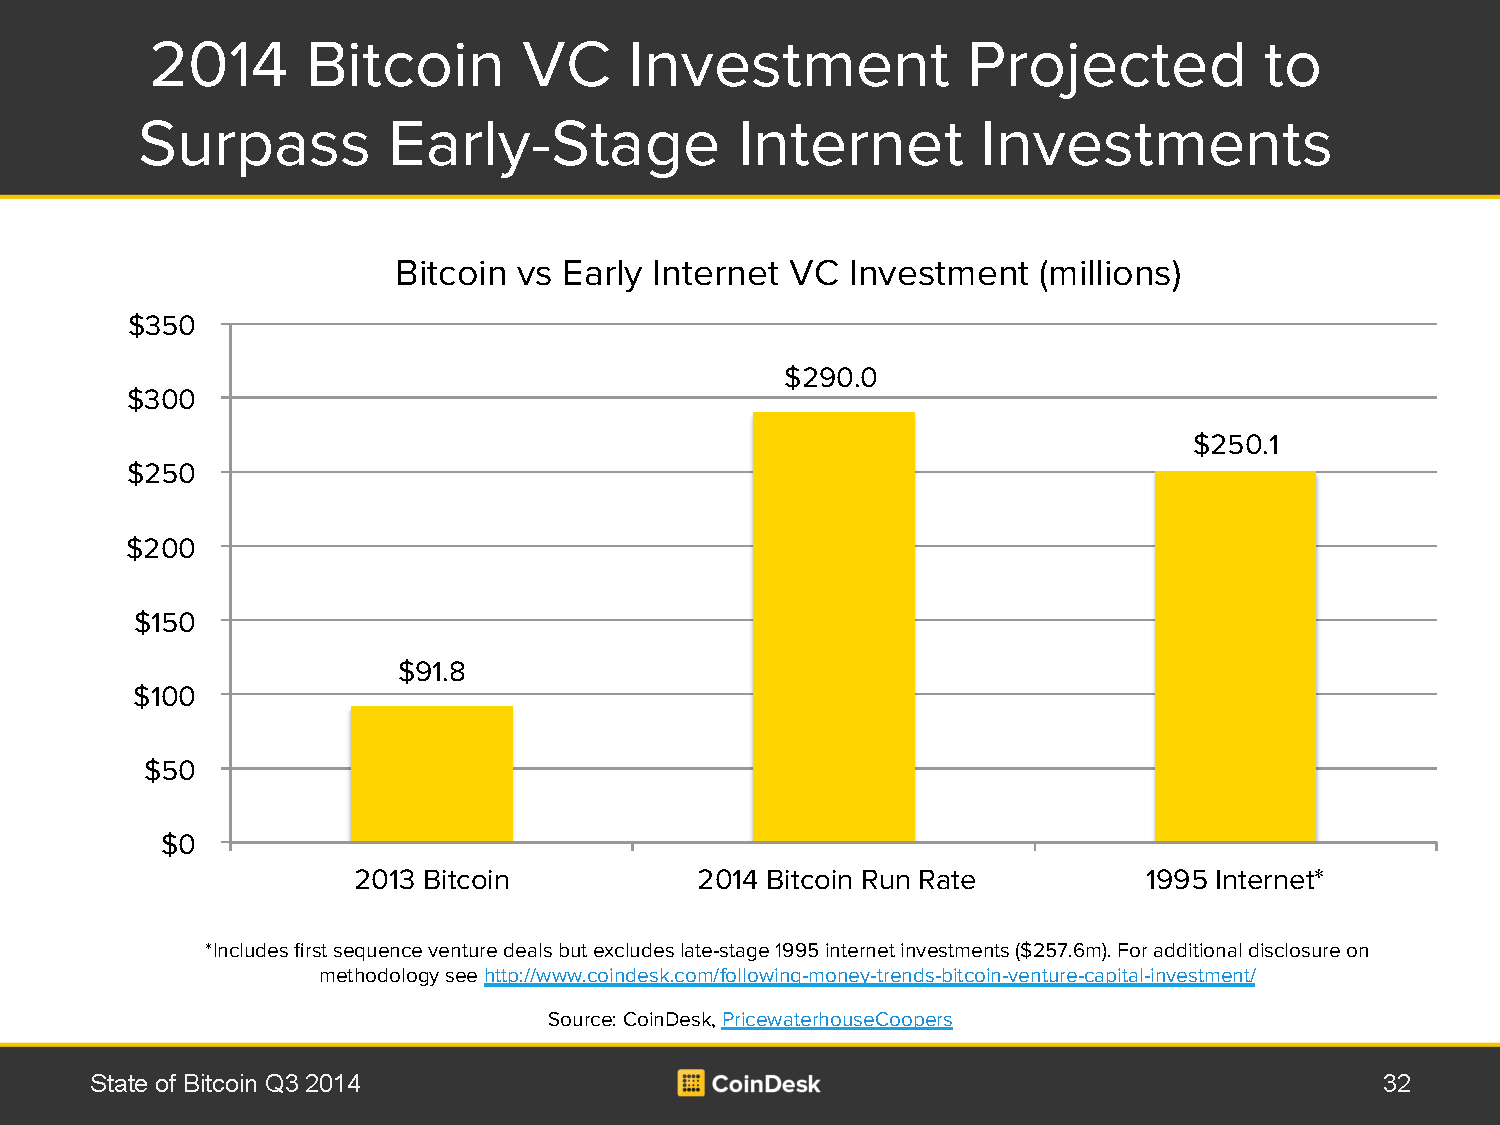
\includegraphics[width=15.649cm,height=8.954cm]{figures/vc.pdf}
\caption{Investimenti in aziende nascenti, o \emph{Startup}, legate al Bitcoin}
\end{figure}

\bigskip

I Filippini cominciano ad usarlo per il mercato miliardario delle
rimesse dei migranti, dove le commissioni sono in ordine dell’8\% medio
(e praticamente il bitcoin le azzera); si stima che la maggior parte
del \textsc{pil} filippino derivi appunto dai soldi che i lavoratori emigrati
mandano alle loro famiglie in patria.

\bigskip

In Kenia, paese africano in forte crescita, già il 40\% del \textsc{pil} è
scambiato via \textsc{sms} con Mpesa, usando telefonini “non smart” per noi
ormai obsoleti. Mpesa è un’azienda monopolista che applica pesanti
tariffe agli scambi e attua atteggiamenti anticompetitivi. Su quel
mercato sta già muovendo i primi passi
Bitpesa\footnote{\url{https://www.bitpesa.co/}}, un interfaccia bitcoin a
Mpesa per le rimesse dei migranti.


\bigskip

Ci sono state valute \emph{iperinflazionate}\footnote{Una valuta che dimezza
il suo potere d'acquisto nell'arco di un mese si dice sia in iperinflazione, è
accaduto di recente in Zimbabwe: \url{http://it.wikipedia.org/wiki/Iperinflazione_nello_Zimbabwe}.}
e ci sono valute a rischio nel mondo, dove il passaggio al bitcoin
permetterebbe alla popolazione libera di effettuare scambi di merci e
servizi in maniera più efficace (in Bangladesh la paura che la gente
fugga nel bitcoin ha fatto sì che il bitcoin sia stato proibito per
legge\footnote{È stato già individuato un nome a questo fenomeno, \emph{Iperbitcoinizzazione}, una sorta di \emph{iperinflazione}
coadiuvata dal bitcoin: \url{http://nakamotoinstitute.org/mempool/hyperbitcoinization/}}).


\section*{Oltre la valuta -- Tecnologia Abilitante}


\lettrine{A}{l di là della valuta in senso stretto}, è la \emph{Blockchain} la vera invenzione 
geniale di Satoshi.
Oltre a tener conto in maniera \emph{Trustless}, cioè \emph{senza
necessità di riporre la fiducia in alcuna autorità centrale}, delle
transazioni bitcoin, è possibile associare dei dati ad una
transazione nella Blockchain. Ora già alcuni di voi avranno intuito che
se si possono scrivere dati in una struttura aperta, pubblica e
crittograficamente protetta come la Blockchain, si sta facendo qualcosa
di nuovo\footnote{Un buon video a questo riguardo lo si trova su
\url{http://youtu.be/YIVAluSL9SU}}.


\bigskip

Certo, si possono scrivere dei dati nel \emph{cloud}\footnote{\url{http://it.wikipedia.org/wiki/Cloud_computing}}, o su un sito web, ma
questi dati non sono inalterabili e non ne è garantita la permanenza. Può incendiarsi un data center
o rompersi l'attrezzatura nonostante le ridondanze prudenziali, ma quello che purtroppo può accadere
è che \emph{il gestore del cloud}, nel quale dobbiamo \emph{necessariamente riporre fiducia}, può, per volontà o disattenzione, rovinare o cancellare i miei
dati. Nella Blockchain questo non può accadere, non serve riporre fiducia in qualcuno, è \emph{Trustless}.

\bigskip

Per la prima volta nell’informatica è stato creato un \emph{Database
Permanente e Inalterabile}.


\bigskip

Che cosa ci possiamo fare? \emph{Decentralizzare} servizi che erano prima
centralizzati o trasformare in \emph{Trustless} una funzione \emph{Trusted}.


\bigskip

Facciamo un esempio semplice, \url{www.proofofexistence.com}, permette di
inserire la firma digitale \ di un documento qualsiasi nella blockchain
per pochi centesimi di euro (5 millibitcoin).


A che cosa può servire? Beh, per \emph{avere una prova matematica} di essere
stati \emph{in possesso di un certo documento} in una certa data, funzione
questa fino ad oggi svolta da un notaio. Grazie alla Blockchain è
svolta senza notaio e ad un costo in paragone risibile.

\bigskip

Bitcoin \emph{è programmabile}. Possiamo usarlo per creare degli \emph{Smart
Contracts}, cioè dei contratti ``elettronici'' nei quali una parte \emph{non può essere
disonesta}: questo significa che non serviranno le funzioni
giuristizionali atte a garantire l’adempimento del contratto (es. la
funzione della polizia per far rispettare il contratto o del tribunale
per sanzionare comportamenti scorretti).

\bigskip

Per fare un esempio di \emph{Smart Contract}, si può pensare alla gestione di fondi aziendali
tramite un portafoglio bitcoin a \emph{multifirma}\footnote{\longurl{http://bitcoin.stackexchange.com/questions/3718/what-are-multi-signature-transactions}}, 
dove un socio da solo può spenderne al
massimo l’1\% al mese, 2 soci potrebbero spenderne il 20\% e dove serve che ci siano
tutte le firme dei soci per spenderne il 100\%.


\bigskip

Possiamo immaginare proprietà digitali applicate ad oggetti
fisici (\emph{Smart Property}), per esempio un’automobile che si accende solo
se la transazione Bitcoin di passaggio di proprietà è presente sulla
Blockchain.


\bigskip

Oppure possiamo anche immaginare distributori automatici che gestiscano direttamente
il denaro in ingresso e facciano gli acquisti per rifornirsi dei
prodotti in esaurimento con parte dei bitcoin incassati, continuando a
\emph{funzionare in autonomia} senza dipendere direttamente dall’azienda che
li gestisce. Una macchina o \emph{un software} non possono \emph{aprire un conto}
corrente tradizionale non essendo persone fisiche o giuridiche, ma
possono scambiare bitcoin e comportarsi da agenti razionali in un
mercato globale.

\begin{figure}
\centering
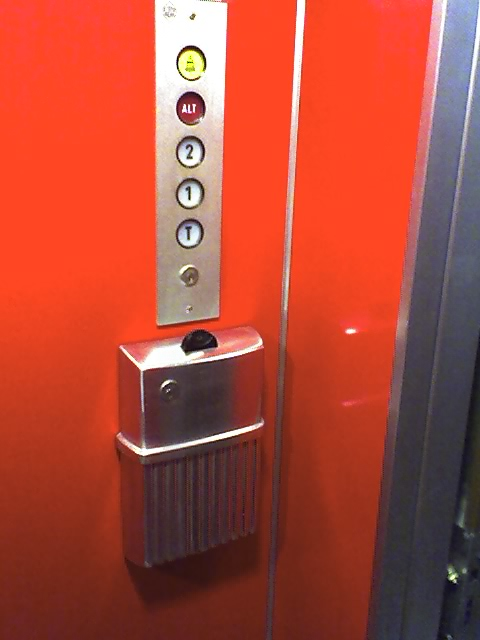
\includegraphics[height=7cm]{figures/elevator.jpg}
\caption{Un ascensore a monetine non programmabili del secolo scorso.}
\end{figure}


\bigskip

\emph{Smart contracts sulla Blockchain} sono un componente
ideale per qualsiasi tipo di \emph{sistema
elettorale} che voglia essere \emph{non manipolabile} da nessuno, pur
mantenendo la caratteristica indispensabile di garantire il voto
segreto all’elettore. A Stalin hanno attribuito la frase: “la gente che
vota non decide nulla, sono quelli che contano i voti a decidere
tutto”, fortunatamente ora c’è una soluzione tecnologica che può
mettere a tacere per sempre le accuse mediatiche di brogli elettorali
che avvengono spesso dopo le
elezioni.\footnote{\longurl{http://motherboard.vice.com/read/bitcoin-could-change-voting-the-way-its-changed-money
}}


\bigskip

Per citare altre cose che bollono in pentola, IBM vuole basare “Adept”,
il cuore del suo progetto per \emph{Internet of Things},\footnote{\url{http://it.wikipedia.org/wiki/Internet_delle_cose}}
sulla Blockchain e
sui protocolli Bitcoin e Bittorrent\footnote{\url{http://goo.gl/AXvA88}}.


\section*{Uno sguardo al futuro}

\lettrine[lines=2]{Q}{ueste applicazioni} sopra elencate sono già possibili con la tecnologia attuale. Che cosa ci
riserverà invece il futuro?

\bigskip

Probabilmente una vasta schiera di \emph{crypto-currencies} tutte scambiabili con
quella per eccellenza, il bitcoin, che saranno progettate per scopi
specifici, anche complessi. Sto parlando di quelle che vengono
attualmente chiamate Appcoin, come le attuali \emph{Namecoin} che permette di
decentralizzare un protocollo internet come il \textsc{dns} o \emph{Ethereum} che punta
a divenire una piattaforma per gli \emph{smart contract}.

\bigskip

Come \emph{divertissement} conclusivo immaginiamo qualcosa ancora più in là nel
futuro e proviamo ad intuire che, magari tra una ventina d’anni, le
\emph{smart-automobili}\footnote{\url{http://it.wikipedia.org/wiki/Google\_driverless\_car
}} che guidano senza pilota \emph{saranno le sole auto a poter circolare
legalmente} nel traffico e immaginiamo di essere a bordo di una di
queste e di avere fretta: bene, l’auto potrà pagare degli \emph{Speedcoin}
alle altre automobili attorno disposte ad accettarli per lasciarci
passare, con il risultato che i viaggiatori con meno urgenza
incasseranno da quelli frettolosi. Sì, saranno le auto stesse che
pagheranno, non il passeggero, avranno la loro riserva digitale di
diverse \emph{Appcoin} per le varie funzioni, intercambiabili in bitcoin e si
pagheranno anche la benzina e la manutenzione da sé. Se hai poca fretta
ti sposterai gratis, altrimenti l’auto guadagnerà su di te che dovrai a
suon di bitcoin sonanti, aumentare la riserva di \emph{Speedcoin} della tua
auto.

C’è già chi ha
teorizzato\footnote{\url
{http://www.slideshare.net/winklevosscap/money-is-broken-its-future-is-not}}
che avverrà una \emph{Singolarità Commerciale}, una specie di punto critico di un sistema, 
quando il volume di denaro
scambiato dalle “cose” (macchine o agenti software che siano)
raggiungerà il volume dei commerci tra umani.

\bigskip

Le reali possibilità sono ancora al di là della nostra immaginazione,
difficile immaginare cosa verrà; sempre che non si sia quel genere di
persone che se fossero vissute negli anni 60 sarebbero state in grado
di immaginare, guardando armadi rumorosi pieni di lucine che un giorno
qualcuno avrebbe giocato ad un gioco di guerra, contro un giocatore
coreano, muovendo le dita su di un vetro sotto il quale appaiono delle
immagini in movimento, ma senza che attori abbiano recitato la parte di
quel film e senza che qualcuno abbia dipinto i fotogrammi.

\bigskip

Buona rivoluzione a tutti. E se non pensate di potervi \emph{giocare un ruolo
attivo}, preparatevi almeno i popcorn e \emph{godetevi lo spettacolo}.


\vfill


\begin{minipage}{.6\linewidth}
Marco Amadori \href{mailto:amadori@fbk.eu}{<amadori@fbk.eu>} \\
Tecnologo e Ricercatore presso la Fondazione Bruno Kessler \url{http://fbk.eu}.
\end{minipage}



\vfill
\begin{footnotesize}da un'idea di divulgazione della scienza per il Blog di \href{http://www.byoblu.org}{ByoBlu}\end{footnotesize}.


\vfill

Questo articolo è distribuito con licenza ``Creative Commons Attribution-ShareAlike 4.0 International Public License'', descritta
all \textsc{URL} \url{http://creativecommons.org/licenses/by-sa/4.0/deed.it}. I sorgenti \LaTeX sono disponibili su 

 \begin{figure}
  \centering

     \qrfig{https://bitcoin.org/it/}
     \qrfig{https://bitcoin.org/bitcoin.pdf} 
     \qrfig{http://youtu.be/YIVAluSL9SU}
     
     \qrfig{http://www.metzdowd.com/pipermail/cryptography/2008-October/014810.html} 
     \qrfig{http://en.wikipedia.org/wiki/Hashcash} 
     \qrfig{http://it.wikipedia.org/wiki/Proof-of-work} 
     
     \qrfig{https://bitcointalk.org/index.php?topic=583.msg11405\#msg11405} 
     \qrfig{https://bitpay.com/} 
     \qrfig{https://greenaddress.it/it/}
     
     \qrfig{https://www.bitpesa.co/} 
     \qrfig{http://motherboard.vice.com/read/bitcoin-could-change-voting-the-way-its-changed-money}
     \qrfig{http://goo.gl/AXvA88}
     
     \qrfig{http://www.slideshare.net/winklevosscap/money-is-broken-its-future-is-not}
     \qrfig{http://it.wikipedia.org/wiki/Google_driverless_car}
     {
     \subcaptionbox{\centering% centering here generates an error
      {\scriptsize Ti è piaciuto questo articolo?} \\ {\ttfamily 1FBKmAA3gFzuT28MpA4EfuqQ5kJEFS9owS}}[.3\linewidth]{%
      \qrcode[height=2.2cm]{1FBKmAA3gFzuT28MpA4EfuqQ5kJEFS9owS}}%
     }
 
 
  \caption{Link principali, citati nell'articolo, in formato QRcode per la scansione con smartphone.}
  \end{figure}



\end{document}

